\documentclass{article}

% packages
\usepackage{amsmath, amsthm, thmtools, amsfonts, amssymb, luacode, catchfile, tikzducks, hyperref, ifthen}
\ifcsname c@kobocompile\endcsname
	\usepackage[a5paper, total={1072pt, 1448pt}, margin=10pt, includeheadfoot]{geometry} % set page margins
\else
	\usepackage[a4paper, margin=50pt, includeheadfoot]{geometry}
\fi
\usepackage[shortlabels]{enumitem}
\usepackage[skip=3pt, indent=0pt]{parskip}

% language
\usepackage[bidi=basic, layout=tabular, provide=*]{babel}
\ifcsname c@english\endcsname
	\babelprovide[main, import]{english}
\else
	\babelprovide[main, import]{hebrew}
	\babelprovide{rl}
\fi
%\babelfont{rm}{Libertinus Serif}
\babelfont{rm}[Renderer=Harfbuzz]{Libertinus Serif}
\babelfont{sf}{Libertinus Sans}
\babelfont{tt}{Libertinus Mono}

% style
\AddToHook{cmd/section/before}{\clearpage}	% Add line break before section
\linespread{1.3}
\setcounter{secnumdepth}{0}		% Remove default number tags from sections, this won't do well with theorems
\AtBeginDocument{\setlength{\belowdisplayskip}{3pt}}
\AtBeginDocument{\setlength{\abovedisplayskip}{3pt}}
\graphicspath{ {../images/} }

% operators
\DeclareMathOperator\cis{cis}
\DeclareMathOperator\Sp{Sp}
\DeclareMathOperator\tr{tr}
\DeclareMathOperator\im{Im}
\DeclareMathOperator\re{Re}
\DeclareMathOperator\diag{diag}
\DeclareMathOperator*\lowlim{\underline{lim}}
\DeclareMathOperator*\uplim{\overline{lim}}
\DeclareMathOperator\rng{rng}
\DeclareMathOperator\Sym{Sym}
\DeclareMathOperator\Arg{Arg}
\DeclareMathOperator\Log{Log}
\DeclareMathOperator\dom{dom}
\DeclareMathOperator\supp{Supp}
\DeclareMathOperator\var{Var}
\DeclareMathOperator\cov{Cov}

% commands
%\renewcommand\qedsymbol{\textbf{מש''ל}}
%\renewcommand\qedsymbol{\fbox{\emoji{lizard}}}
\newcommand{\Aa}[0]{\mathcal{A}}
\newcommand{\Bb}[0]{\mathcal{B}}
\newcommand{\CC}[0]{\mathbb{C}}
\newcommand{\Cc}[0]{\mathcal{C}}
\newcommand{\EE}[0]{\mathbb{E}}
\newcommand{\FF}[0]{\mathbb{F}}
\newcommand{\Ff}[0]{\mathcal{F}}
\newcommand{\Ii}[0]{\mathcal{I}}
\newcommand{\Gg}[0]{\mathcal{G}}
\newcommand{\Ll}[0]{\mathcal{L}}
\newcommand{\Mm}[0]{\mathcal{M}}
\newcommand{\NN}[0]{\mathbb{N}}
\newcommand{\Nn}[0]{\mathcal{N}}
\newcommand{\PP}[0]{\mathbb{P}}
\newcommand{\Pp}[0]{\mathcal{P}}
\newcommand{\QQ}[0]{\mathbb{Q}}
\newcommand{\RR}[0]{\mathbb{R}}
\newcommand{\Rr}[0]{\mathcal{R}}
\newcommand{\Ss}[0]{\mathcal{S}}
\newcommand{\TT}[0]{\mathbb{T}}
\newcommand{\Uu}[0]{\mathcal{U}}
\newcommand{\Vv}[0]{\mathcal{V}}
\newcommand{\Ww}[0]{\mathcal{W}}
\newcommand{\ZZ}[0]{\mathbb{Z}}
\newcommand{\acts}[0]{\circlearrowright}
\newcommand{\explain}[2] {
	\begin{flalign*}
		 && \text{#2} && \text{#1}
	\end{flalign*}
}
\newcommand{\maketitleprint}[0]{ \begin{center}
	%\begin{tikzpicture}[scale=3]
	%	\duck[graduate=gray!20!black, tassel=red!70!black]
	%\end{tikzpicture}	
	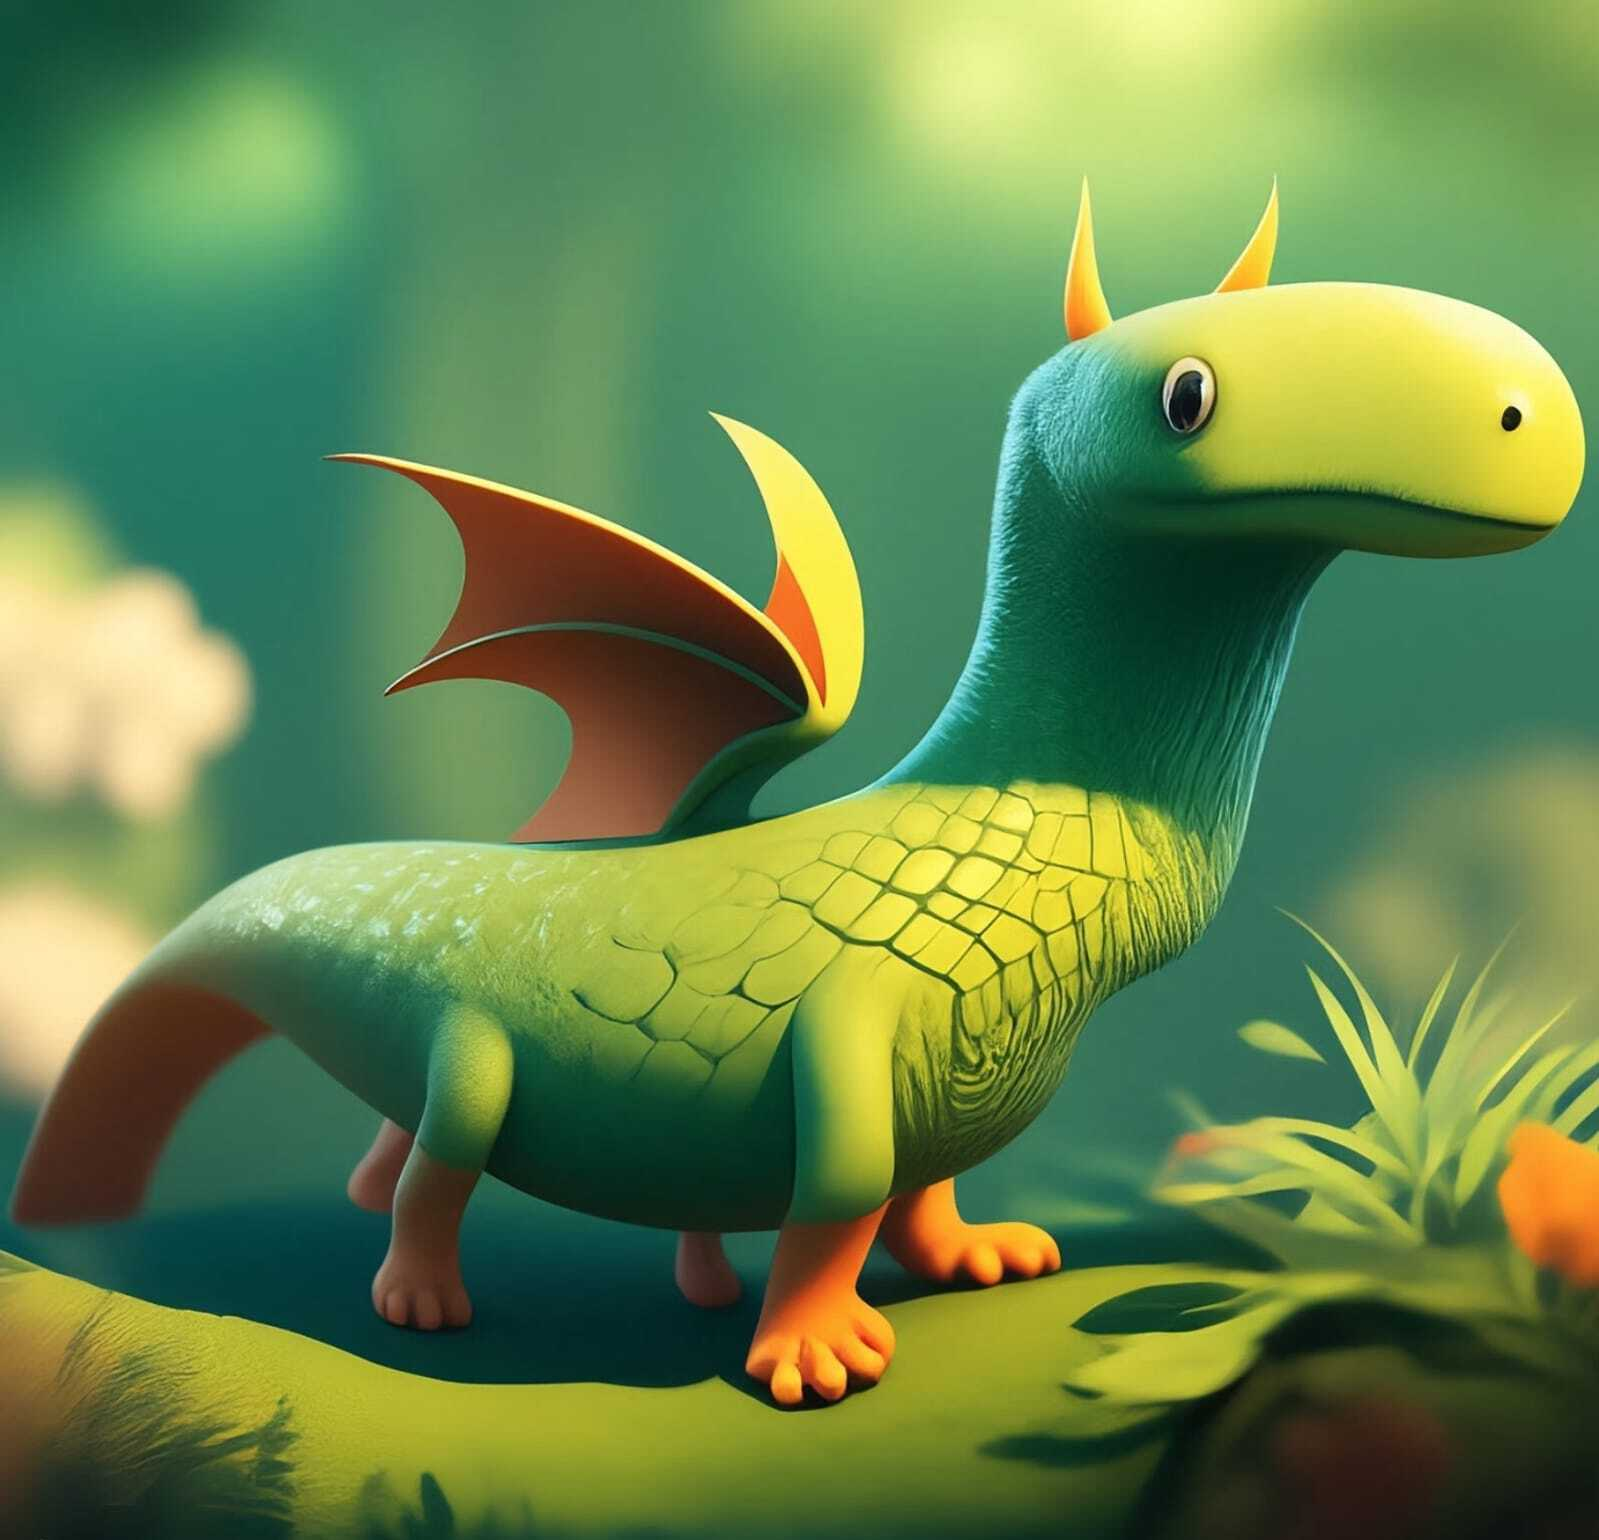
\includegraphics[width=6cm]{cover}
\end{center}
}

% theorem commands
\newtheoremstyle{c_remark}
	{}	% Space above
	{}	% Space below
	{}% Body font
	{}	% Indent amount
	{\bfseries}	% Theorem head font
	{}	% Punctuation after theorem head
	{.5em}	% Space after theorem head
	{\thmname{#1}\thmnumber{ #2}\thmnote{ \normalfont{\text{(#3)}}}}	% head content
\newtheoremstyle{c_definition}
	{3pt}	% Space above
	{3pt}	% Space below
	{}% Body font
	{}	% Indent amount
	{\bfseries}	% Theorem head font
	{}	% Punctuation after theorem head
	{.5em}	% Space after theorem head
	{\thmname{#1}\thmnumber{ #2}\thmnote{ \normalfont{\text{(#3)}}}}	% head content
\newtheoremstyle{c_plain}
	{3pt}	% Space above
	{3pt}	% Space below
	{\itshape}% Body font
	{}	% Indent amount
	{\bfseries}	% Theorem head font
	{}	% Punctuation after theorem head
	{.5em}	% Space after theorem head
	{\thmname{#1}\thmnumber{ #2}\thmnote{ \text{(#3)}}}	% head content

\ifcsname c@english\endcsname
	\theoremstyle{plain}
	\newtheorem{theorem}{Theorem}[section]
	\newtheorem{lemma}[theorem]{Lemma}
	\newtheorem{proposition}[theorem]{Proposition}
	\newtheorem*{proposition*}{Proposition}
	%\newtheorem{corollary}[theorem]{אין חלופה עברית}

	\theoremstyle{definition}
	\newtheorem{definition}[theorem]{Definition}
	\newtheorem*{definition*}{Definition}
	\newtheorem{example}{Example}[section]
	\newtheorem{exercise}{Exercise}[section]

	\theoremstyle{remark}
	\newtheorem*{remark}{Remark}
	\newtheorem*{solution}{Solution}
	\newtheorem{conclusion}[theorem]{Conclusion}
	\newtheorem{notation}[theorem]{Notation}
\else
	\theoremstyle{c_plain}
	\newtheorem{theorem}{משפט}[section]
	\newtheorem{lemma}[theorem]{למה}
	\newtheorem{proposition}[theorem]{טענה}
	\newtheorem*{proposition*}{טענה}
	%\newtheorem{corollary}[theorem]{אין חלופה עברית}

	\theoremstyle{c_definition}
	\newtheorem{definition}[theorem]{הגדרה}
	\newtheorem*{definition*}{הגדרה}
	\newtheorem{example}{דוגמה}[section]
	\newtheorem{exercise}{תרגיל}[section]

	\theoremstyle{c_remark}
	\newtheorem*{remark}{הערה}
	\newtheorem*{solution}{פתרון}
	\newtheorem{conclusion}[theorem]{מסקנה}
	\newtheorem{notation}[theorem]{סימון}
\fi

% Questions related commands
\newcounter{question}
\setcounter{question}{1}
\newcounter{sub_question}
\setcounter{sub_question}{1}

\ifcsname c@english\endcsname
	\newcommand{\question}[1][0]{
		\ifthenelse{#1 = 0}{}{\setcounter{question}{#1}}
		\section{Question \arabic{question}}
		\addtocounter{question}{1}
		\setcounter{sub_question}{1}
	}

	\newcommand{\subquestion}[1][0]{
		\ifthenelse{#1 = 0}{}{\setcounter{sub_question}{#1}}
		\subsection{Part \alph{sub_question}}
		\addtocounter{sub_question}{1}
	}
\else
	\newcommand{\question}[1][0]{
		\ifthenelse{#1 = 0}{}{\setcounter{question}{#1}}
		\section{שאלה \arabic{question}}
		\addtocounter{question}{1}
		\setcounter{sub_question}{1}
	}

	\newcommand{\subquestion}[1][0]{
		\ifthenelse{#1 = 0}{}{\setcounter{sub_question}{#1}}
		\subsection{סעיף \localecounter{letters.gershayim}{sub_question}}
		\addtocounter{sub_question}{1}
	}
\fi

% import lua and start of document
\directlua{common = require ('../common')}

\GetEnv{AUTHOR}

% headers
\author{\AUTHOR}
\date\today

\title{פתרון מטלה 09 --- תורת ההסתברות (1), 80420}

\DeclareMathOperator{\Supp}{Supp}

\begin{document}
\maketitle
\maketitleprint{}

\question{}
נחסום על־ידי אי־שוויון מרקוב ובעזרת אי־שוויון צ'בישב את ההסתברות שלתמורה אקראית על $[n]$ יש לפחות $k$ נקודות שבת.
\begin{solution}
	נגדיר $X$ מספר נקודות השבת וכן $X_i$ שבמספר ה־$i$ יש נקודת שבת.
	מאי־שוויון מרקוב
	\[
		\PP(X \ge k)
		\le \frac{\EE(X)}{k}
	\]
	ובתרגול 8 ראינו ש־$\EE(X) = 1$ ולכן
	\[
		\PP(X \ge k)
		\le \frac{1}{k}
	\]
	ניזכר כי באותו תרגול ראינו גם ש־$\var(X) = 1$,
	לפי אי־שוויון צ'בישב
	\[
		\PP(X \ge k)
		= \PP(X - 1 \ge k - 1)
		= \PP(|X - \EE(X)| \ge k - 1)
		\le \frac{\var(X)}{{(k - 1)}^2}
		= \frac{1}{{(k - 1)}^2}
	\]
	וכמובן אסימפטוטית זהו חסם טוב בהרבה.
\end{solution}

\question{}
בכיתה $n$ תלמידים. ימי ההולדת שלהם בלתי־תלויים וכל יום הולדת מתפלג אחיד על פני שנה כלשהי. \\
יהי $X$ משתנה מקרי שסופר את זוגות התלמידים שחולקים יום הולדת.

\subquestion{}
נחשב את תוחלת $X$.
\begin{solution}
	בשיעור 14 ביצענו את החישוב הדרוש, והתקבל שאם יש $m$ ימים בשנה הנתונה, אז
	\[
		\EE(X) = \binom{n}{2} \frac{1}{m}
	\]
\end{solution}

\subquestion{}
יהיו $i, j, k, l \in [n]$ כך ש־$\{i, j\} \ne \{k, l\}$, נראה שהמאורע ש־$i, j$ חולקים יום הולדת בלתי תלוי במאורע ש־$k, l$ חולקים יום הולדת.
\begin{proof}
	נניח ש־$X_\iota$ המשתנה המקרי שמייצג שלתלמיד ה־$\iota \in [n]$ יש יום הולדת ביום מסוים, אז $X_i \sim U([m])$. \\
	נחלק למקרים על ארבעת התלמידים הנתונים. \\
	במקרה הראשון $i \ne j \ne k \ne l$ ולכן חוסר התלות נובע מחוסר התלות של $X_\iota$. \\
	מקרה נוסף הוא המקרה ש־$i = j \ne k = l$, כלומר בחרנו שני תלמידים בלבד, אז ישירות מחוסר התלות הנתון של ימי ההולדת גם הפעם מאורעות אלה בלתי תלויים. \\
	נשאר אפוא לבדוק את המקרה (ללא הגבלת הכלליות) ש־$i = k$ אך $j \ne l$,
	\[
		\PP(X_i = X_j, X_k = X_l)
		= \PP(X_i = X_j, X_i = X_l)
		= \PP(X_i = X_j = X_l = \alpha)
		= \PP(X_i = \alpha) \PP(X_j = \alpha) \PP(X_l = \alpha)
	\]
	כפי שרצינו להראות (כאשר $\PP(X_\iota = X_\iota) = 1$).
\end{proof}

\subquestion{}
נחשב את השונות של $X$.
\begin{solution}
	לצורך חישוב זה נגדיר $X_{i, j}$ המשתנה המקרי ש־$i$ ול־$j$ יש יום הולדת משותף, לכן $X_{i, j} \sim Ber(\frac{1}{m})$. \\
	נובע גם ש־$X = \sum_{i = 1}^{n} \sum_{j = i + 1}^{n} X_{i, j}$.
	\begin{align*}
		\var(X)
		& = \cov(X, X) \\
		& = \left( \sum_{1 \le i < j \le n} \left( \sum_{\substack{1 \le k < l \le n \\ \{i, j\} \ne \{k, l\}}} \cov(X_{i, j}, X_{l, k}) \right) \right)
		+ \left( \sum_{1 \le i < j \le n} \left( \sum_{\substack{1 \le k < l \le n \\ \{i, j\} = \{k, l\}}} \cov(X_{i, j}, X_{l, k}) \right) \right) \\
		& = \left( \sum_{1 \le i < j \le n} \left( \sum_{\substack{1 \le k < l \le n \\ \{i, j\} \ne \{k, l\}}} 0 \right) \right) + \left( \sum_{1 \le i < j \le n}  \cov(X_{i, j}, X_{i, j}) \right) \\
		& = 0 + \left( \sum_{1 \le i < j \le n}  \var(X_{i, j}) \right) \\
		& = \sum_{1 \le i < j \le n} \frac{1}{m} (1 - \frac{1}{m}) \\
		& = \frac{n(n - 1)(m - 1)}{2m^2}
	\end{align*}
\end{solution}

\subquestion{}
נחסום על־ידי אי־שוויון צ'בישב את ההסתברות שבכיתה בת 30 תלמידים יש שלושה זוגות שחולקים יום הולדת.
\begin{solution}
	מהנתונים $n = 30, m = 365, \lambda = 3$, ומאי־שוויון צ'בישב
	\begin{align*}
		\PP(X \ge \lambda)
		& = \PP(X - \EE(X) \ge \lambda - \EE(X)) \\
		& = \PP(\left\lvert X - \binom{n}{2} \frac{1}{m} \right\rvert \ge \lambda - \binom{n}{2} \frac{1}{m}) \\
		& \le \frac{\var(X)}{\lambda - \binom{n}{2} \frac{1}{m}} \\
		& = \frac{\frac{n(n - 1)(m - 1)}{2m^2}}{\lambda - \binom{n}{2} \frac{1}{m}} \\
		& = \frac{n(n - 1)(m - 1)}{2m^2 \lambda - 2m \binom{n}{2}}
	\end{align*}
	נציב ונקבל $\PP(X \ge 3) \lessapprox 0.657$, כלומר הסיכוי שיש לפחות שלושה זוגות חסום על־ידי כשני שלישים.
\end{solution}

\question{}
אליס בוחרת באקראי מספר שלם ב־$[100]$ ובוב מנחש באקראי את המספר שהיא בחרה. \\
לאחר מכן בוב משלם לאליס את ריבוע ההפרש בין המספר שאליס בחרה לבין המספר שבוב ניחש.

\subquestion{}
נחשב את המספר שעל בוב לנחש כדי למזער את תוחלת התשלום שלו לאליס.
\begin{solution}
	נגדיר $b$ המספר שבחר בוב, וכן $X_a \sim U([100])$ה מספר שבחרה אליס, ולבסוף $Y = {(X_a - b)}^2$ הכסף שבוב ישלם לאליס בסוף.
	\[
		\EE(Y)
		= \EE(X_a^2) - 2b \EE(X_a) + b^2
		= (\sum_{i \in [100]} \frac{i^2}{100}) - 2b \frac{100 + 1}{2} + b^2
		= 3383.5 - 101b + b^2
	\]
	ולכן נגדיר $f(b) = 3383.5 - 101b + b^2$ ונגזור,
	\[
		f'(b) = 2b - 101,
		\qquad
		f''(b) = 2
	\]
	ולכן בנקודה $b = 50.5$ מקבלת הפונקציה מינימום, וזהו גם המספר שעל בוב לבחור (כאשר אם אסור לו לבחור מספר לא שלם כי הוא לא מתחכם, אז הבחירה 50 או 51 יהיו טובות באותה המידה).
\end{solution}

\subquestion{}
נניח שבוב אכן בוחר במדיניות שממזערת את תוחלת התשלום שלו כמו בסעיף הקודם. \\
אליס משחקת בהוגנות ומציעה לבוב לשלם מראש סכום מסוים, נחשב את הסכום שעל אליס לשלם כדי שתוחלת ההפסד של בוב תהיה אפס.
\begin{solution}
	בסעיף הקודם מצאנו ש־$Y = {(X_a - 50.5)}^2$ המשתנה המקרי שמייצג את ההפסד של בוב במקרה שבו הוא בוחר מספר שימזער את ההפסד שלו.
	מהחישוב שעשינו גם נובע
	\[
		\EE(Y)
		= 3383.5 - 101 \cdot 50.5 + 50.5^2
		= 833.25
	\]
	כלומר תוחלת ההפסד של בוב היא $833.25$, ואם אליס תשלם לו מראש בדיוק את הסכום הזה לפני תחילת הסיבוב, אז בהתאם תוחלת ההפסד שלו תתאפס (ישירות מלינאריות התוחלת).
\end{solution}

\question{}
יהי אספן פוגים שבכל יום קונה חטיף במבה בו יש פוג בהתפלגות אחידה מבין $n$ סוגי פוגים.

\subquestion{}
נסמן ב־$Y_k$ את המשתנה המקרי שמתאר את היום הראשון בו יש לאספן $k$ פוגים שונים. \\
נראה שהמשתנים המקריים ${\{Y_k - Y_{k - 1}\}}_{1 < k \le n}$ הם בלתי־תלויים ומתפלגים גאומטרית עם פרמטר $1 - \frac{k - 1}{n}$.
\begin{proof}
	מטעמי שימוש בנוסחת ההסתברות השלמה מספיק שנבחן את המקרה שבו כלל המשתנים המקריים מוגדרים, אז
	\begin{align*}
		\PP(Y_2 - Y_1 = s_1, \dots, Y_n - Y_{n - 1} = s_{n - 1})
		& = \PP(Y_1 = 1, Y_2 - Y_1 = s_1, \dots, Y_n - Y_{n - 1} = s_{n - 1}) \\
		& = \PP(Y_1 = 1, Y_2 = 1 + s_1, \dots, Y_n = 1 + \cdots + s_{n - 1}) \\
		& = \PP(Y_2 = 1 + s_1, \dots, Y_n = 1 + \cdots + s_{n - 1}) \\
		& = \sum_{\{c_1, \dots, c_n\} \in S_n} \PP(\forall 1 \le i \le n, X_1, \dots, X_{s_i} \in \{c_1, \dots, c_{i - 1}\}, X_{1 + s_i} = c_i) \\
		& = \sum_{\{c_1, \dots, c_n\} \in S_n} \prod_{1 < i \le n} \PP(X_1, \dots, X_{s_i} \in \{c_1, \dots, c_{i - 1}\}, X_{1 + s_i} = c_i) \\
		& = n! \prod_{1 < i \le n} \PP(X_1, \dots, X_{s_i} \in [i - 1]) \PP(X_{s_i + 1} = i) \\
		& = n! \prod_{1 < i \le n} {(\frac{i - 1}{n})}^{s_i} \frac{1}{n} \\
		& = (n - 1)! \prod_{1 < i \le n} {(\frac{i - 1}{n})}^{s_i}
	\end{align*}
	וכן
	\begin{align*}
		\PP(Y_k - Y_{k - 1} = s_k)
		& = \PP(X_{Y_{k - 1}}, \dots, X_{Y_k - 1} \in [k - 1], X_{Y_k} \in \{k, \dots, n\}) \\
		& = \PP(X_{Y_{k - 1}} \in [k - 1]) \cdots \PP(X_{Y_k - 1} \in [k - 1]) \PP(X_{Y_k} \in \{k, \dots, n\}) \\
		& = {(\frac{k - 1}{n})}^{Y_k - Y_{k - 1} - 1} \cdot \frac{n - k + 1}{n} \\
		& = {(\frac{k - 1}{n})}^{s_k - 1} \cdot \frac{n - k + 1}{n}
	\end{align*}
	כלומר $Y_k - Y_{k - 1} \sim Geo(1 - \frac{k - 1}{n})$ ומכפלת המשתנים הללו היא בדיוק התוצאה שחישבנו קודם לכן, לכן הם בלתי־תלויים ומתפלגים גאומטרית.
\end{proof}

\subquestion{}
נחשב את תוחלת מספר הימים שיעבור עד שלאספן יהיו כלל הפוגים.
\begin{solution}
	אנו רוצים לחשב את $Y_n$, אך זה בתורו מקיים $Y_n = Y_n - Y_{n - 1} + Y_{n - 1} - Y_{n - 2} + \cdots + Y_2 - Y_1 + Y_1$.
	לכן מלינאריות התוחלת, אי־התלות וההתפלגות
	\[
		\EE(Y_n)
		= \EE(Y_n - Y_{n - 1}) + \cdots + \EE(Y_2 - Y_1) + \EE(Y_1)
		= 1 + \sum_{k = 2}^{n} \frac{1}{1 - \frac{k - 1}{n}}
		= 1 + n \sum_{l = 0}^{n - 2} \frac{1}{l + 1}
		= 1 + n \sum_{l = 1}^{n - 1} \frac{1}{l}
	\]
	נבחין כי מטור טיילור של $\log$ כאשר $n \to \infty$ גם $\EE(Y_n) \to 1 + n \log(1 + n)$ ולכן אסימפטוטית התוחלת מתנהגת כמו $n \log n$.
\end{solution}

\subquestion{}
נחשב את שונות מספר הימים שיעברו עד שלאספן יהיו כלל הפוגים.
\begin{solution}
	תחילה נחשב את השונות של $Y_k - Y_{k - 1}$ לכל $2 \le k \le n$, זוהי כמובן שונות של התפלגות גאומטרית ולכן
	\[
		\var(Y_k - Y_{k - 1})
		= \frac{1 - (1 - \frac{k - 1}{n})}{{(1 - \frac{k - 1}{n})}^2}
	\]
	נשתמש בחוסר התלות ובתכונות השונות והשונות המשותפת,
	\begin{align*}
		\var(Y_n)
		& = \var(Y_n - 1) \\
		& = \cov(Y_n - Y_{n - 1} + \cdots Y_2 - Y_1, Y_n - Y_{n - 1} + \cdots Y_2 - Y_1) \\
		& = \sum_{k = 1}^{n} \cov(Y_k - Y_{k - 1}, Y_k - Y_{k - 1}) + 2\sum_{1 \le k < l \le n} \cov(Y_k - Y_{k - 1}, Y_l - Y_{l - 1}) \\
		& = \sum_{k = 1}^{n} \var(Y_k - Y_{k - 1}) + 2\sum_{1 \le k < l \le n} 0 \\
		& = \sum_{k = 1}^{n} \var(Y_k - Y_{k - 1}) \\
		& = \sum_{l = 0}^{n} \frac{\frac{l}{n}}{{\left(1 - \frac{l}{n}\right)}^2} \\
		& \xrightarrow[n \to \infty]{} \int_0^{1 - \frac{1}{n}} \frac{x}{{(1 - x)}^2}\ dx \\
		& = n + \log \frac{1}{n} \\
		& = o(n^2)
	\end{align*}
	ולכן הפונקציה מתנהגת אסימפטוטית כמו $n^2$.
\end{solution}

\subquestion{}
נראה שאחרי $C n \log n$ ימים ההסתברות שלאספן יש את כל הפוגים שואפת ל־1 אם $C > 1$ ושואפת ל־$0$ אם $C < 1$.
\begin{proof}
	\[
		\PP(Y_n \ge C n \log n)
		\le \frac{\EE(Y_n)}{C n \log n}
		= \frac{o(n \log n)}{C n \log n}
		= \frac{o(n \log n)}{n \log(n^C)}
	\]
	ומכאן נוכל להסיק את האמור.
\end{proof}

\question{}
נחשב כמה קטנה יכולה להיות השונות המשותפת $\cov(X_i, X_j)$ אם ידוע ש־$X_1, \dots, X_n$ הם משתנים מקריים המתפלגים $Ber(\frac{1}{2})$, וכי השונות המשותפת של כולם שוות. \\
נראה דוגמה שבה המינימום מתקבל.
\begin{solution}
	נגדיר $X = \sum_{i = 1}^{n} X_i$ וכן נגדיר $\cov(X_1, X_2) = K$, אז
	\[
		\EE(X)
		= \sum_{i = 1}^{n} \EE(X_i)
		= \frac{n}{2}
	\]
	וכן מתכונות השונות,
	\[
		\var(X)
		= \sum_{i = 1}^n \cov(X, X_i)
		= \sum_{i = 1}^n \sum_{j = 1}^n \cov(X_i, X_j)
		= (n^2 - n) K + \frac{n}{4} \cdot n
	\]
	אבל שונות היא אי־שלילית ולכן
	\[
		(n^2 - n) K + \frac{n}{4} \cdot n \ge 0
		\iff
		K \ge \frac{1}{4(1 - n)}
	\]
	ומצאנו ערך מינימלי לשונות המשותפת.

	נגדיר $n = 2$ וכן $X_1 \sim Ber(\frac{1}{2})$ ו־$X_2 = 1 - X_1$, כלל ההנחות מתקיימות באופן ריק וכן מתכונות השונות המשותפת
	\[
		\cov(X_1, X_2)
		= \cov(X_1, 1 - X_1)
		= \cov(X_1, - X_1)
		= - \cov(X_1, X_1)
		= - \var(X_1)
		= - p (1 - p)
		= -\frac{1}{4}
	\]
	ומהצד השני
	\[
		\frac{1}{4(1 - n)}
		= -\frac{1}{4}
	\]
	ומצאנו שהמינימום אכן מתקבל.
\end{solution}

\end{document}
